\section{Corrente Alternada}

\frame{
	\frametitle{Introdução a C.A.}
	\begin{block}{Corrente Contínua (C.C.)}
		\begin{itemize}
			\item Fontes de corrente e tensão possuem valores constantes, i.e., não variam com o tempo.
		\end{itemize}
	\end{block}

	\begin{block}{Corrente Alternada (C.A.)}
		\begin{itemize}
			\item A intensidade da fonte varia de uma forma definida.
		\end{itemize}
	\end{block}
}

\frame{
	\frametitle{C.C. x C.A.}
%	\setmyunit{0.1ex}
	
	\centering
	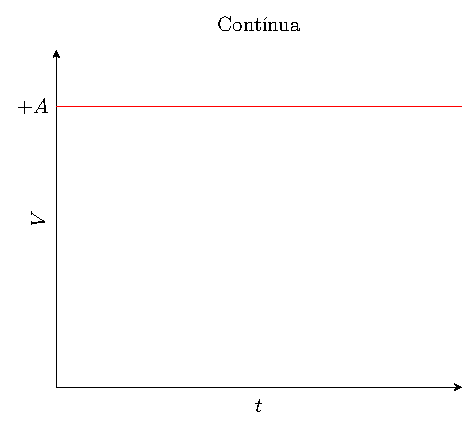
\includegraphics[page=1,height=0.9\textheight]{Figuras/Ch11/sinefunc.pdf}
%	\centerline{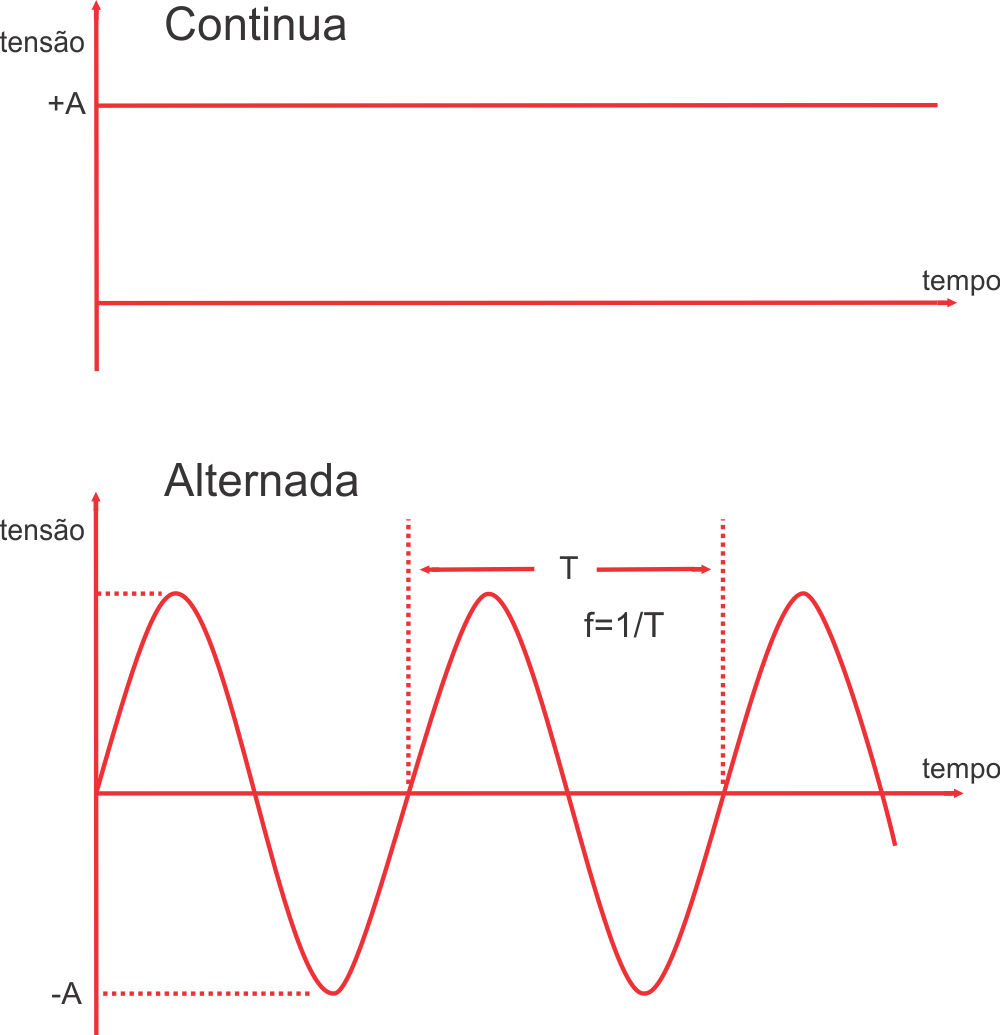
\includegraphics[width=0.6\linewidth]{Figuras/Ch11/ccca.png}}
}

\frame{
	\frametitle{C.C. x C.A.}
	%	\setmyunit{0.1ex}
	
	\centering
	\includegraphics[page=2,height=0.9\textheight]{Figuras/Ch11/sinefunc.pdf}
	%	\centerline{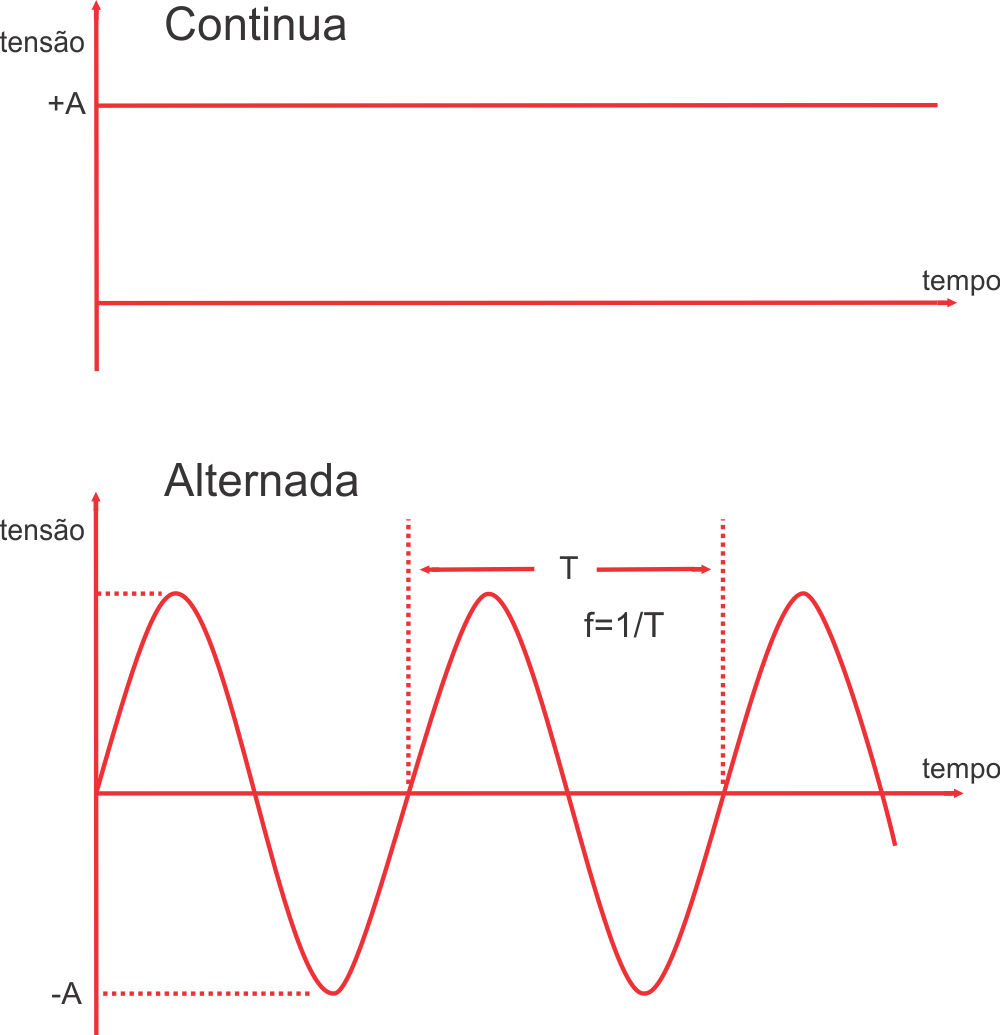
\includegraphics[width=0.6\linewidth]{Figuras/Ch11/ccca.png}}
}

\frame{
	\frametitle{Corrente Alternada}
	\centerline{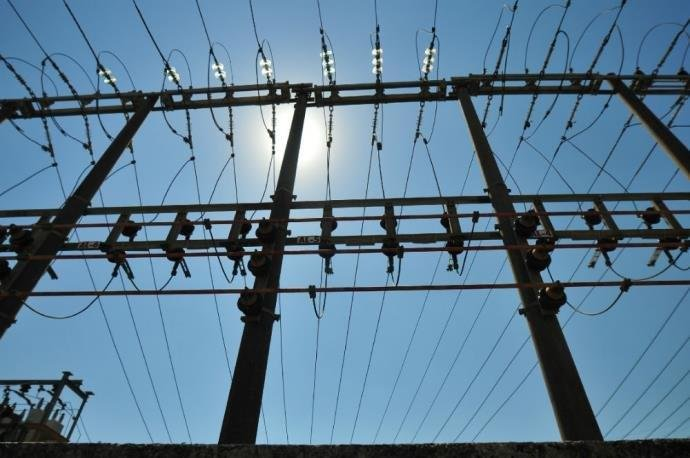
\includegraphics[width=0.9\linewidth]{Figuras/Ch11/ca.jpg}}
}

\frame{
	\frametitle{Formas de ondas alternadas}
	\centerline{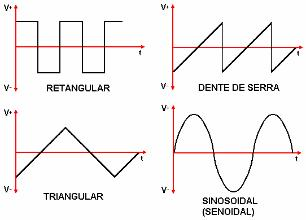
\includegraphics[width=0.7\linewidth]{Figuras/Ch11/ondas.jpg}}
}

\frame{
	\frametitle{Geração de C.A.}
	\begin{block}{Princípio de funcionamento}
		\begin{itemize}
			\item Dispositivo que produz uma Força Eletromotriz (f.e.m.) pela variação do número de linhas de fluxo (linhas de força) magnético, $\vec{\Phi}$, que atravessam uma bobina de fio.
		\end{itemize}
	\end{block}
	\centerline{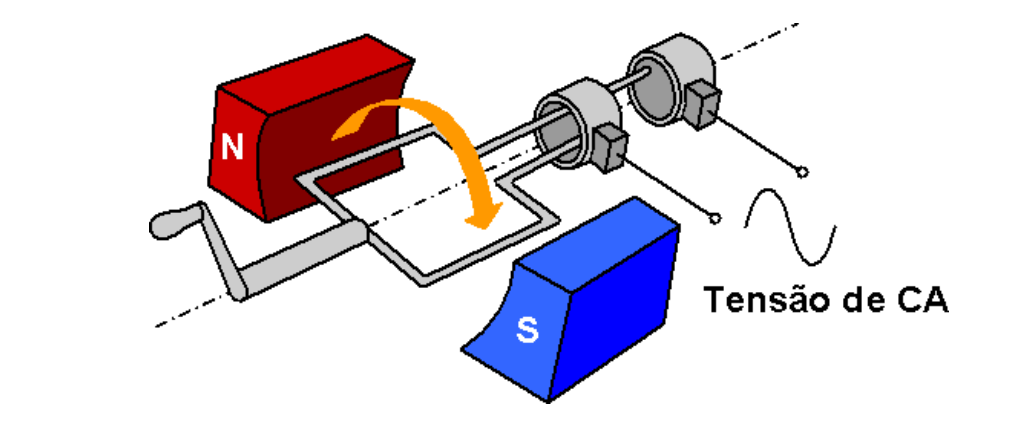
\includegraphics[width=0.8\linewidth]{Figuras/Ch11/gerador.PNG}}
}

\frame{
	\frametitle{Princípio da indução eletromagnética}
	\begin{block}{Lei de Faraday}
		$$\vec{E_m} = - N \dfrac{\Delta \vec{\Phi}}{\Delta t}$$
	\end{block}
	\centerline{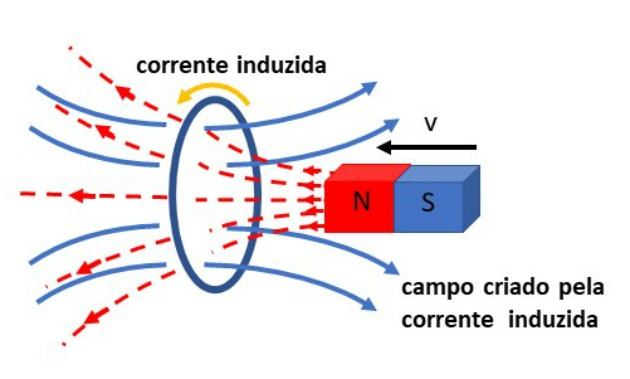
\includegraphics[width=0.8\linewidth]{Figuras/Ch11/faraday.jpg}}
}

\frame{
	\frametitle{Sentido da corrente induzida}
	\begin{block}{Lei de Lenz}
		A corrente elétrica induzida em um circuito possui um sentido tal que o campo magnético que ela cria tende a contrariar a variação de fluxo magnético que a originou.
	\end{block}
	\centerline{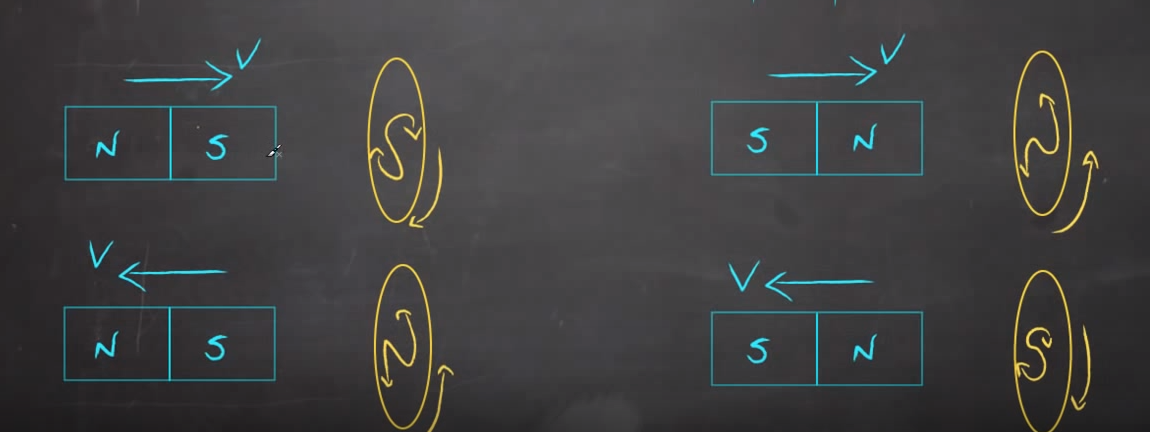
\includegraphics[width=0.8\linewidth]{Figuras/Ch11/lenz.PNG}}
}

\frame{
	\frametitle{Geração de C.A.}
	\begin{block}{Princípio de funcionamento}
		\begin{itemize}
			\item No gerador, a bobina está sob a influência de campo magnético. A densidade do fluxo magnético, $\vec{B}$, é constante e $\vec{\Phi} = B \cdot A_{ef}$, assim $\vec{\Phi}$ é proporcional à área efetiva da espira. A medida que a espira gira em ângulos diferentes, há uma alteração da área efetiva.
		\end{itemize}
	\end{block}
	\centerline{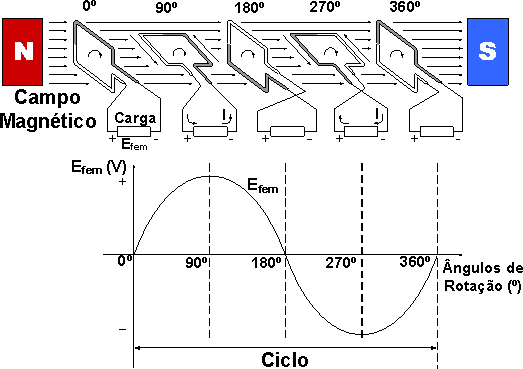
\includegraphics[width=0.6\linewidth]{Figuras/Ch11/area.png}}
}

\frame{
	\frametitle{Definições - Onda senoidal}
	\centering
	\includegraphics[page=3,height=0.6\textheight]{Figuras/Ch11/sinefunc}
	
	\vspace{-0.2cm}
	\begin{block}{Parâmetros}
		\begin{itemize}
			\item \textbf{Valor instantâneo ($ \bm{v(t)} $)}: amplitude de uma forma de onda em um instante de tempo qualquer.
			\item \textbf{Valor pico a pico ($ \bm{U_{pp}} $)}: é a diferença entre os valores dos picos positivo e negativo.
		\end{itemize}
	\end{block}
}

\frame{
	\frametitle{Definições - Onda senoidal}
	\centering
	\includegraphics[page=3,height=0.6\textheight]{Figuras/Ch11/sinefunc}
	
	\vspace{-0.2cm}
	\begin{block}{Parâmetros}
		\begin{itemize}
			\item \textbf{Amplitude de pico ($ \bm{A_m} $)}: valor máximo de uma forma de onda em relação ao valor médio.
			\item \textbf{Valor de pico ($ \bm{V_m} $)}: valor máximo instantâneo de uma função medido a partir do nível zero volt.
		\end{itemize}
	\end{block}
}

\frame{
	\frametitle{Definições - Onda senoidal}
	\centering
	\includegraphics[page=3,height=0.5\textheight]{Figuras/Ch11/sinefunc}
	
	\vspace{-0.2cm}
	\begin{block}{Parâmetros}
		\begin{itemize}
			\item \textbf{Período ($ \bm{T} $)}: intervalo de tempo entre repetições sucessivas de uma forma de onda periódica.
			\item \textbf{Ciclo}: parte de uma forma de onda contida em um intervalo de tempo igual a um período.
			\item \textbf{Frequência ($ \bm{f} $)}: número de ciclos que ocorrem em $1$ s. [Hz]
		\end{itemize}
	\end{block}
}

\frame{
	\frametitle{Definições - Onda senoidal}
	\begin{block}{Importante}
		A senoide é a única forma de onda alternada cuja forma não se altera ao ser aplicada a um circuito contendo resistores, indutores e capacitores.
	\end{block}
	\centerline{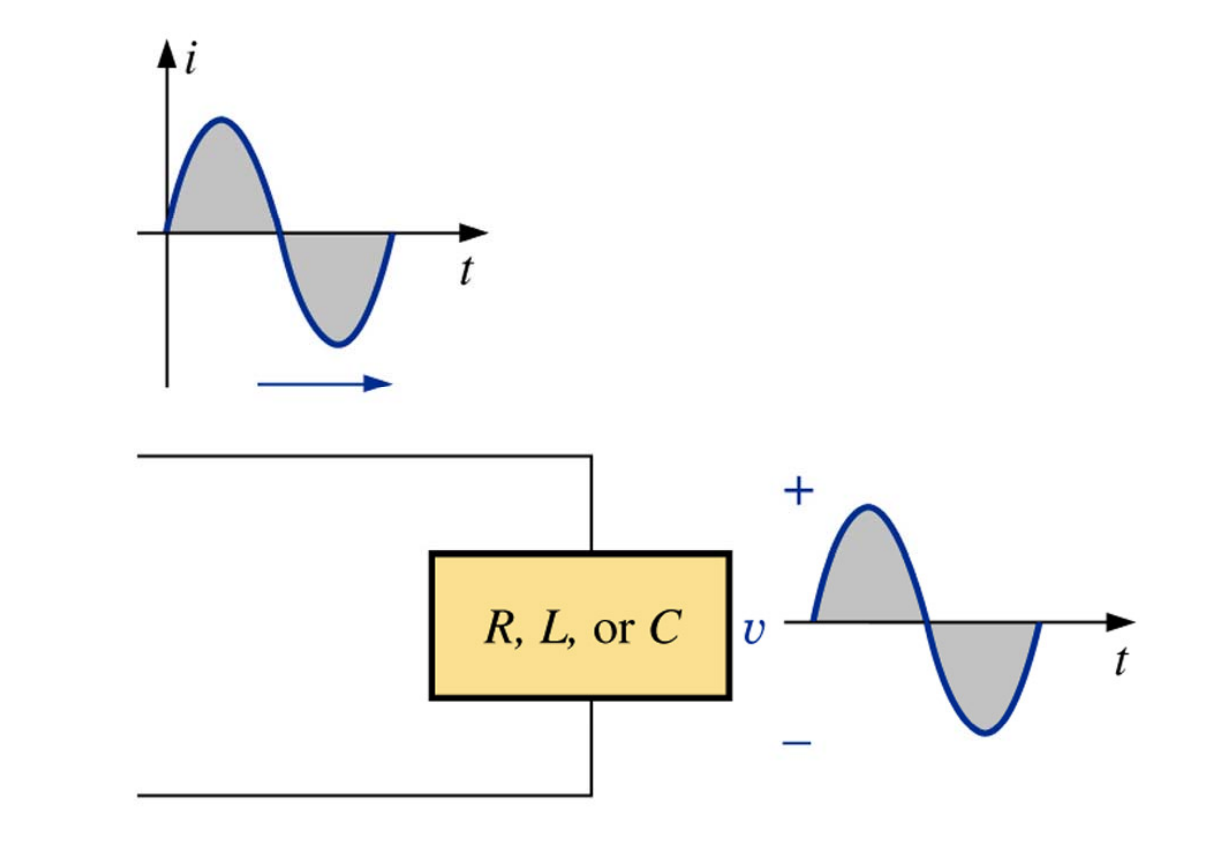
\includegraphics[width=0.7\linewidth]{Figuras/Ch11/senoidemantem.PNG}}
}

\frame{
	\frametitle{Conversões matemáticas}
	\begin{block}{Algumas relações}
		$$\SI{1}{\radian} = \ang{57,3}$$ \\
		$$\SI{2\pi}{\radian}= \ang{360}$$ \\
		$$\text{radianos} = \dfrac{\pi}{\ang{180}} \times \text{graus}$$ \\
		$$\text{graus} = \dfrac{\ang{180}}{\pi} \times \text{radianos}$$ \\
		$$\omega = \frac{2\pi}{T} \implies \omega = 2\pi f$$
	\end{block}
}

\frame{
	\frametitle{Expressão geral de sinais senoidais}
	\begin{block}{Importante}
		$$A(t) = A_m \sen(\omega t \pm \theta)$$
		
		\begin{itemize}
			\item $A_m$: amplitude da senoide
			\item $\omega$: frequência angular em rad/s
			\item $\theta$: ângulo de defasagem
		\end{itemize}
	\end{block}
}

\frame{
	\frametitle{Relação de fase}
	\begin{block}{Avanço}
		$$A(t) = A_m \sen(\omega t + \theta)$$
	\end{block}
	\centerline{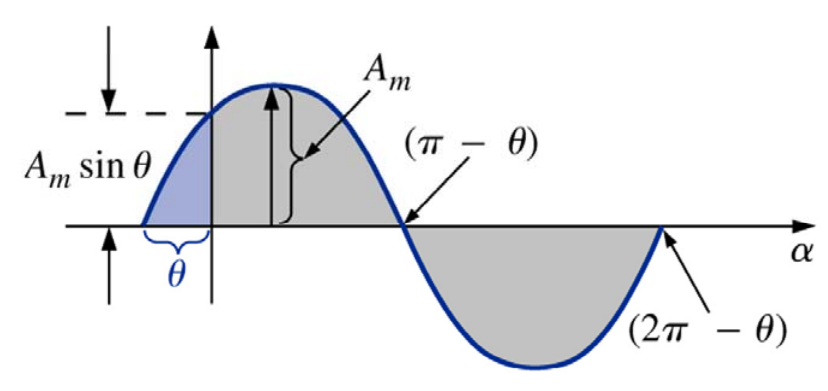
\includegraphics[width=0.7\linewidth]{Figuras/Ch11/avanco.PNG}}
}

\frame{
	\frametitle{Relação de fase}
	\begin{block}{Atraso}
		$$A(t) = A_m \sen(\omega t - \theta)$$
	\end{block}
	\centerline{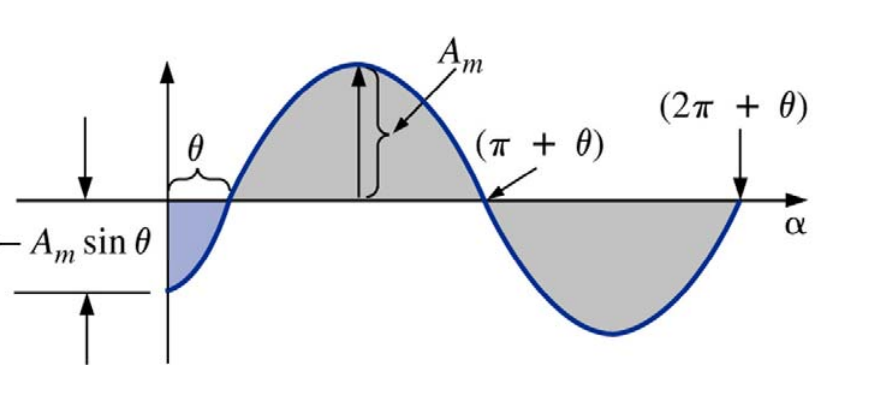
\includegraphics[width=0.7\linewidth]{Figuras/Ch11/atraso.PNG}}
}

\frame{
	\frametitle{Relação de fase}
	\centerline{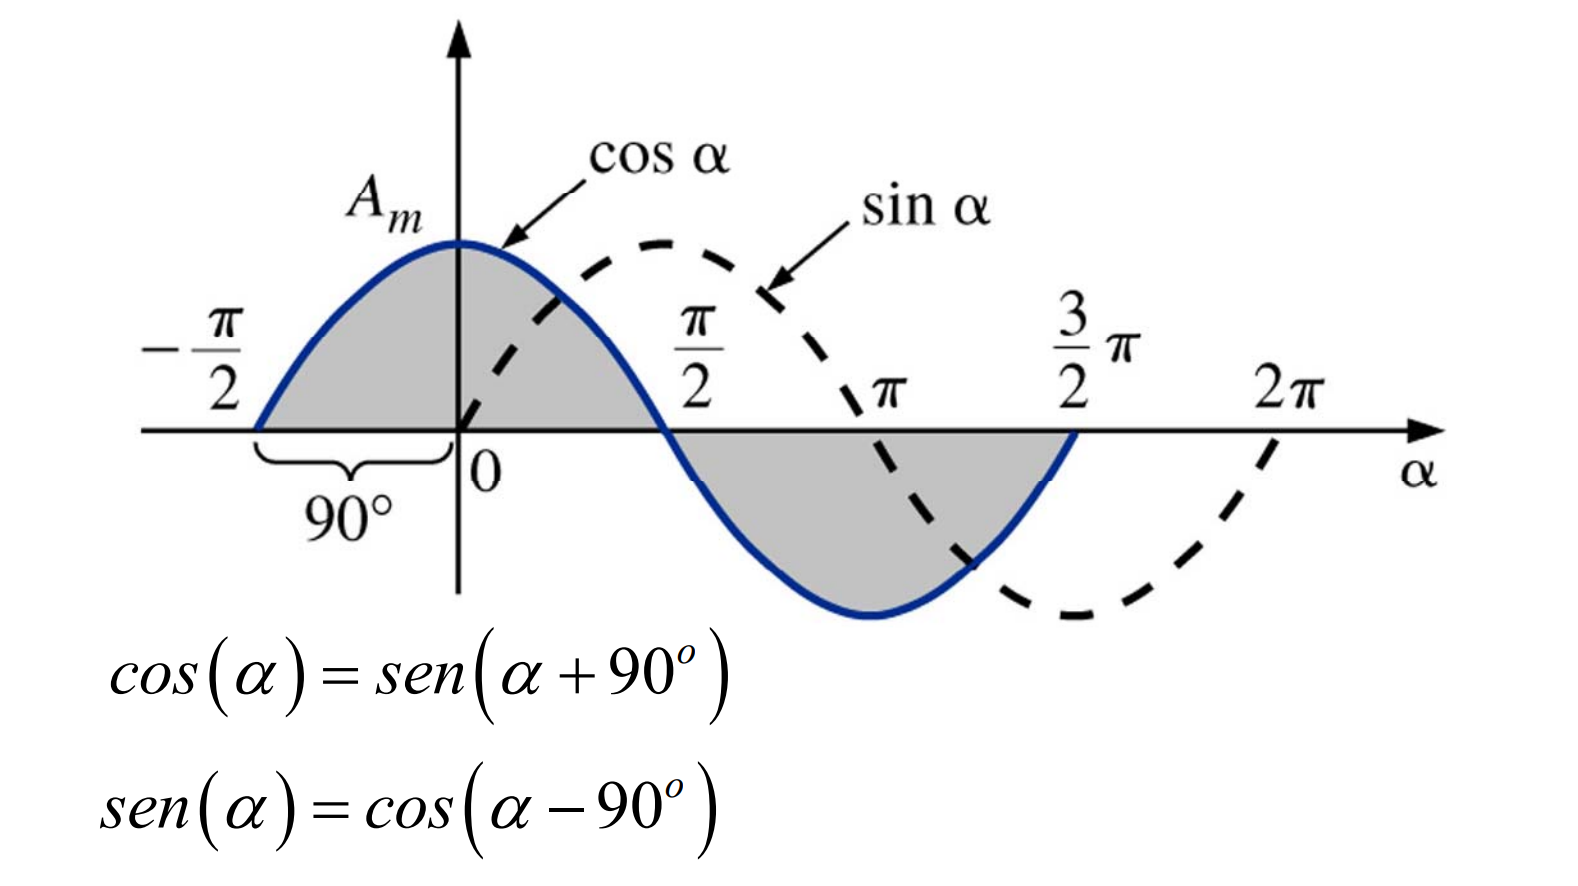
\includegraphics[width=0.9\linewidth]{Figuras/Ch11/sincos.PNG}}
}

\frame{
	\frametitle{Valor médio}
	\begin{block}{Relação matemática}
		$$\text{valor médio} = \frac{\text{soma algébrica da curva}}{\text{comprimento da curva}}$$
	\end{block}
	\centerline{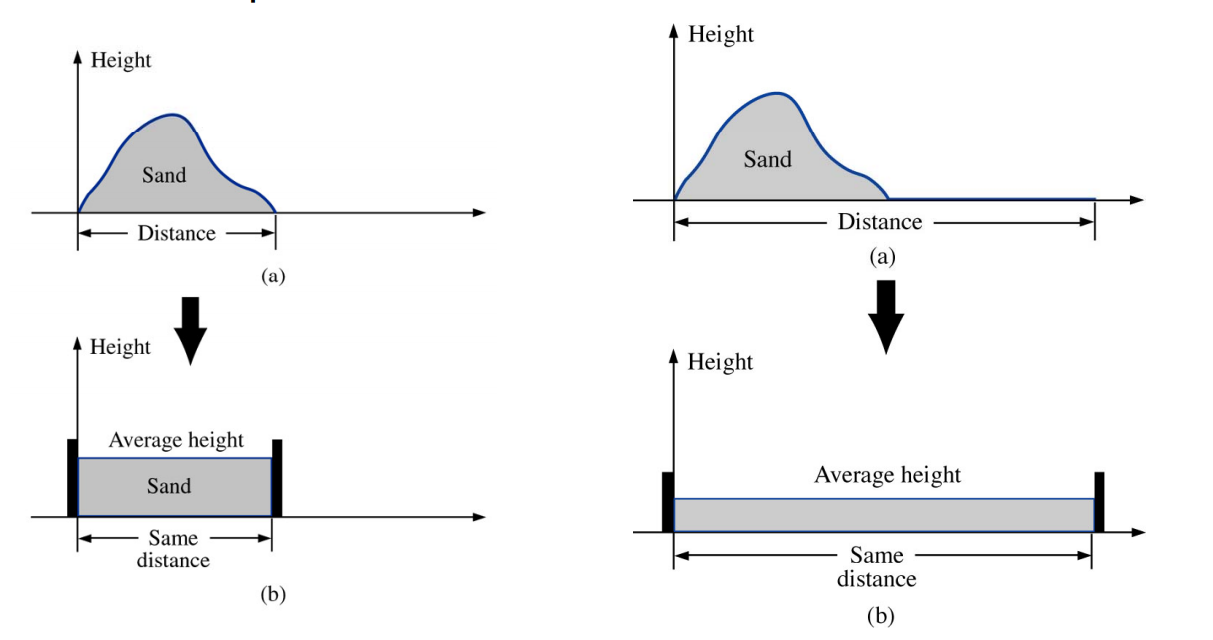
\includegraphics[width=0.9\linewidth]{Figuras/Ch11/valormedio.PNG}}
}

\frame{
	\frametitle{Valor médio}
	\begin{block}{Importante}
		O valor médio de uma função senoidal pura para um período completo é sempre zero.
	\end{block}

	\centering
	\includegraphics[page=4,height=0.7\textheight]{Figuras/Ch11/sinefunc}
%	\centerline{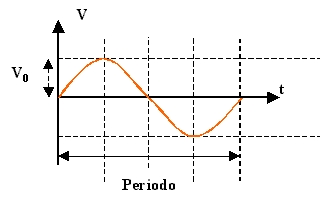
\includegraphics[width=0.8\linewidth]{Figuras/Ch11/valormedio2.JPG}}
}

\frame{
	\frametitle{Exemplo - Valor médio}
	\centerline{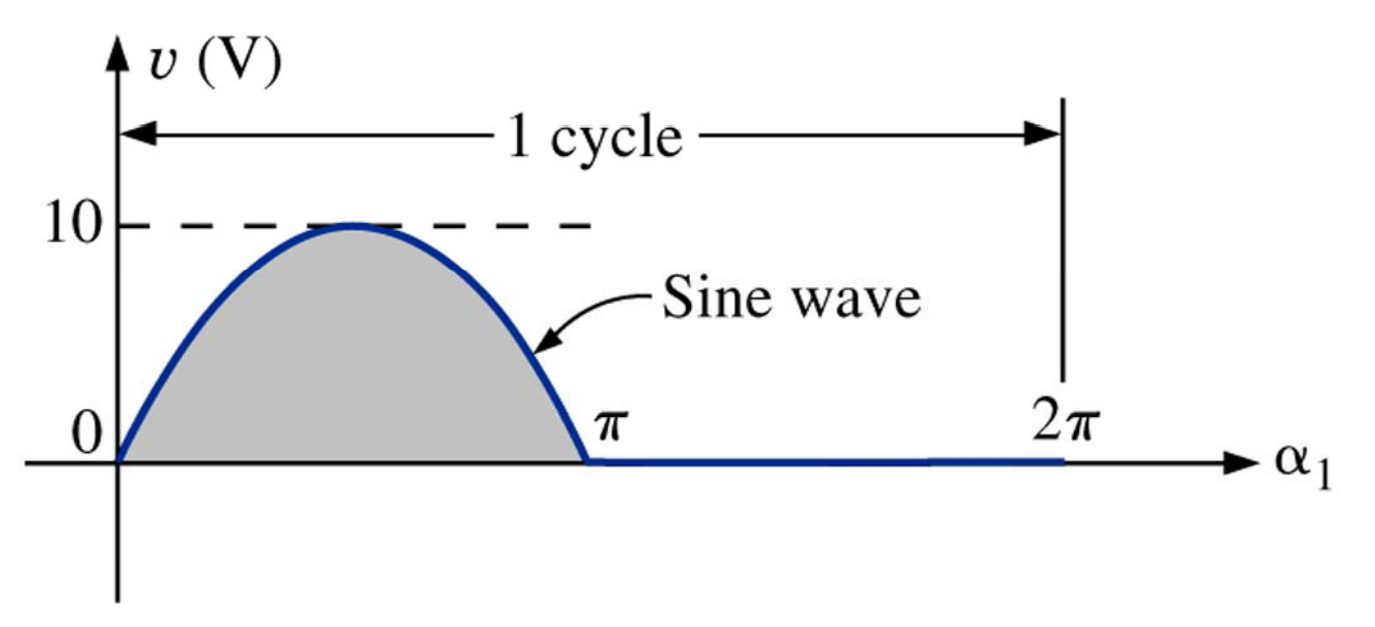
\includegraphics[width=0.8\linewidth]{Figuras/Ch11/valormedio3.PNG}}
	\begin{block}{Aproximação da área: $\text{área} = 2 V_0$}
		$\text{valor médio} = \dfrac{2 V_0 + 0}{2 \pi} = \dfrac{\num{2.10}}{2 \pi} = \SI{3.18}{\volt}$
	\end{block}
}

\frame{
	\frametitle{Valor eficaz ou RMS}
	\begin{block}{Definição}
		É definido como o valor equivalente de uma tensão alternada (C.A.) que produziria o mesmo
		trabalho que uma tensão contínua (C.C.).
	\end{block}
	\centerline{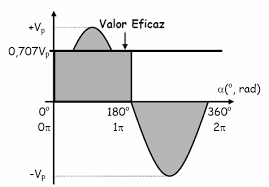
\includegraphics[width=0.7\linewidth]{Figuras/Ch11/valoreficaz.png}}
}

\frame{
	\frametitle{Valor eficaz ou RMS}
	\begin{block}{Fórmula}
		$$I_{rms} = \dfrac{I_m}{\sqrt{2}}$$ \\
		$$V_{rms} = \dfrac{V_m}{\sqrt{2}}$$
	\end{block}
	\centerline{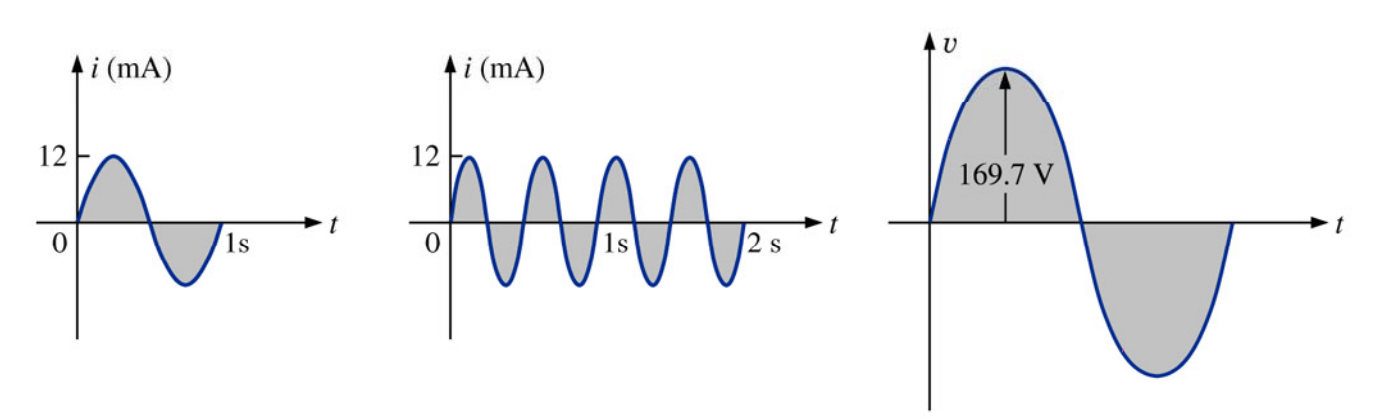
\includegraphics[width=1.1\linewidth]{Figuras/Ch11/valoreficaz2.PNG}}
}

\section*{Exercícios}

\frame{
	\frametitle{Exercícios}
	\begin{block}{}
		01. Uma fonte contínua de \SI{120}{\volt} fornece \SI{3.6}{\watt} à carga. Determine os valores de pico da tensão aplicada $E_m$ e da corrente $I_m$ para que a fonte alternada forneça a mesma potência a uma carga idêntica.

		\vspace{1cm}

		02. Qual a relação de fase entre as formas de onda senoidais? \\
		(a) $i = -\sen(\omega t + \ang{30}) \text{e} v = 2 \sen(\omega t + \ang{10})$ \\
		(b) $i = -2 \cos(\omega t - \ang{30}) \text{e} v = 3 \sen(\omega t - \ang{150})$

		\vspace{1cm}

		03. Determine a amplitude, a fase, a frequência, o período e a frequência angular da senoide $v(t) = 12 \cos(50t + \ang{10})$

	\end{block}
}

\section*{Referências}

\frame{
	\frametitle{Referências e Exercícios Complementares}
	\begin{itemize}
		\item ALEXANDRE, Charles K.; SADIKU, Matthew N. O. Fundamentos de Circuitos Elétricos. 5. ed. Porto Alegre: AMGH, 2013.
	\end{itemize}
	%\centering{\alert{Página 36 - \textbf{1.6.1 até 1.6.5, 1.6.17 até 1.6.19}}} \\
	\centering{\alert{Lista de exercícios 11}}
}